Pneumatic mechanism is also a potential solution. Pneumatic method can be done with air or fluid and the advantage of it is that the power source is divorced from the actuator.
Power, in the form of pressurized air, is routed via small pipes and readily converted into the motion of a sliding pin using an elastic membrane.
This feature of separation of power source and functional module make pneumatic design promising in terms of forming a large-area dense array shape display.
However, one big challenge of pneumatic design is how to efficiently control large number of cells without sacrifice of portability.

The group proposed a fluidic logic system design (figure \ref{fig:pneumatic-schema}) to solve this problem and the prototype showed positive results in the earlier tests.
Blitab managed to release their fluid-based product a few years ago but their product is still in pre-order state and never entered the market formally.
While very promising, we could not replicate it within our budgetary constraints.
\begin{figure}\centering
    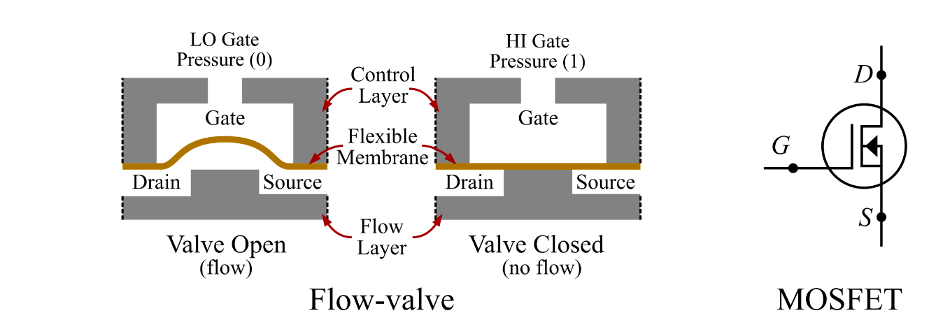
\includegraphics[width=0.6\textwidth]{figures/pneumatic-schema.png}
\caption{Cross-sectional views of a pressure-based fluidic valve in the open and closed states.}
\label{fig:pneumatic-schema}
\end{figure}